\documentclass{beamer}
\usepackage{graphicx}
\usepackage{color}
\usepackage{setspace}
%\usepackage{enumitem}
%\setlist[itemize]{leftmargin=*}
\newcommand{\figpath}{../Figures/}
\newcommand{\red} [1]{\textcolor{red}{#1}}
\newcommand{\blue}[1]{\textcolor{blue}{#1}}
\newcommand{\black}[1]{\textcolor{black}{#1}}
\newcommand{\slidecite}[3]{[{\sc {#1} {\it {#2}} {#3}}]}
\newcommand{\pdf}{\operatorname{pdf}}

%-------------- aliases -----------------------
\newcommand{\ie}{{\it i.e.\,}}
\newcommand{\vs}{{\it vs.\,}}
\newcommand{\eg}{{\it e.g.\,}}
\newcommand{\nablab}{{\boldsymbol{\nabla}}}
\newcommand{\Upsilonb}{{\boldsymbol{\Upsilon}}}
\newcommand{\Ab}{\mathbf{A}}
\newcommand{\As}{\mathsf{A}}
\newcommand{\ab}{\mathbf{a}}
\newcommand{\db}{\mathbf{d}}
\newcommand{\eb}{\mathbf{e}}
\newcommand{\fb}{\mathbf{f}}
\newcommand{\Ep}{\mathbb{E}}
\newcommand{\yb}{\mathbf{y}}
\newcommand{\dx}{\Delta\mathbf{x}}
\newcommand{\xb}{\mathbf{x}}
\newcommand{\rb}{\mathbf{r}}
\newcommand{\pb}{\mathbf{p}}
\newcommand{\Xb}{\mathbf{X}}
\newcommand{\Xs}{\mathsf{X}}
\newcommand{\Rb}{\mathbf{R}}
\newcommand{\cluster}{\mathcal{C}}
\newcommand{\Ib}{\mathbf{I}}
\newcommand{\Is}{\mathsf{I}}
\newcommand{\Pb}{\mathbf{P}}
\newcommand{\Pp}{\mathbb{P}}
\newcommand{\Ub}{\mathbf{U}}
\newcommand{\Us}{\mathsf{U}}
\newcommand{\Vb}{\mathbf{V}}
\newcommand{\Vs}{\mathsf{V}}
\newcommand{\Ws}{\mathsf{W}}
\newcommand{\Db}{\mathbf{D}}
\newcommand{\Ds}{\mathsf{D}}
\newcommand{\Mb}{\mathbf{M}}
\newcommand{\spn}{\operatorname{span}}
\newcommand{\tr}{\operatorname{tr}}
\newcommand{\RMSD}{\operatorname{RMSD}}
\newcommand{\SVD}{\operatorname{SVD}}
\newcommand{\Ball}{\mathcal{B}}
\newcommand{\argmin}{\operatorname{argmin}}
\newcommand{\argmax}{\operatorname{argmax}}


\begin{document}
\title{
\red{\underline{\small TMS 143$^\text{rd}$ Annual Meeting, San Diego, Feb. 16-20, 2014}} \\
{\bf Smart use of Density Functional Theory calculations to drive Newtonian dynamics}
\\
\vspace{0.05in}
\black{
\large
{\bf Reese Jones} and Mickey Shaughnessy \\
{\it \small  Sandia National Laboratories and Synopsis, Inc.}
}
\vspace{-0.05in}
\begin{center}
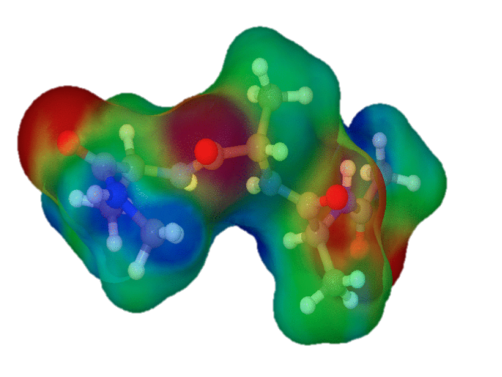
\includegraphics[width=0.5\textwidth]{molecule_forces.pdf} \\
\fbox{
\begin{minipage}[h!]{0.85\textwidth}
\begin{spacing}{0.5}
{\tiny
Sandia   National        Laboratories    is      a       multi­‐program   laboratory     managed         and     operated        by      Sandia   Corporation,   a       wholly  owned   subsidiary      of      Lockheed         Martin         Corporation,    for     the     U.S.    Department      of       Energy's       National        Nuclear         Security        Administration   under  contract        DE-­‐AC04-­‐94AL85000. }
\end{spacing}
\vspace{0.1in}
\end{minipage}
}
\end{center}
}
\date{}

%%%%%%%%%%%%%%%%%%%%%%%%%%%%%%%%%%%%%%%%%%%%%%%%%%%%%%%%%%%%%%%%%%%%%%%%%%%%
\frame{\titlepage}
%%%%%%%%%%%%%%%%%%%%%%%%%%%%%%%%%%%%%%%%%%%%%%%%%%%%%%%%%%%%%%%%%%%%%%%%%%%%
\frame{\frametitle{Outline}
\begin{minipage}[h!]{0.65\textwidth}

{\bf Motivation:}
\red{\it compositionally} and \red{\it structurally complex} materials and processes: e.g. deposition and radiation damage, require the dynamic simulation of \red{\it large} atomic systems with \red{\it multiple} interspecies interactions.

\begin{center}

\fbox{
Outline: 

\vspace{0.1in}
\begin{minipage}[h!]{0.7\textwidth}

\tableofcontents
\end{minipage}
}
\end{center}

\begin{center}
\red{please ask questions}
\end{center}
\end{minipage}\hfill%
\begin{minipage}[h!]{0.30\textwidth}
\begin{center}

atomic deposition
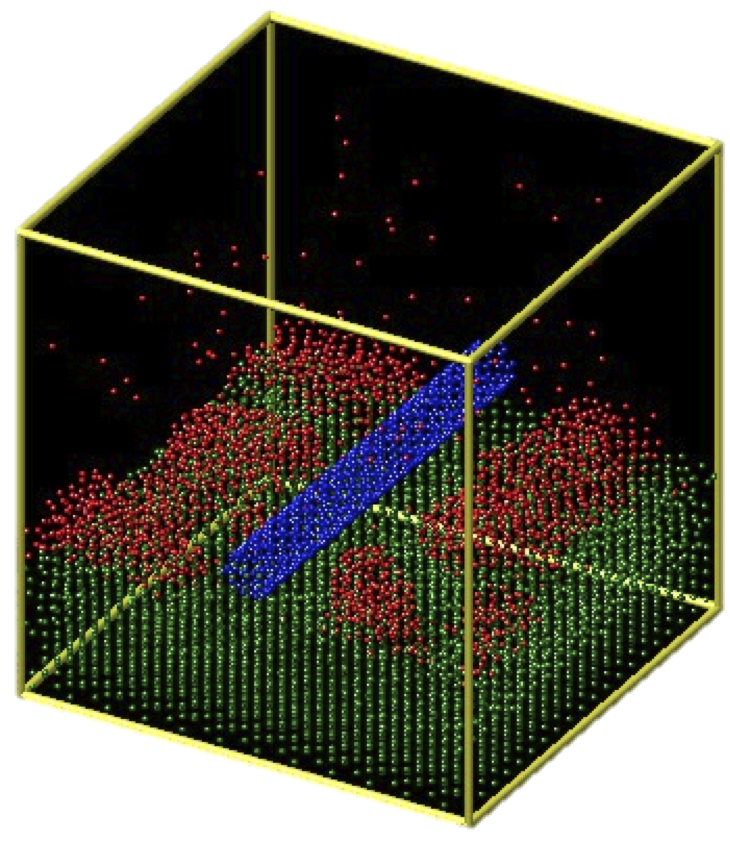
\includegraphics[width=0.95\textwidth]{deposit.png} 

radiation damage
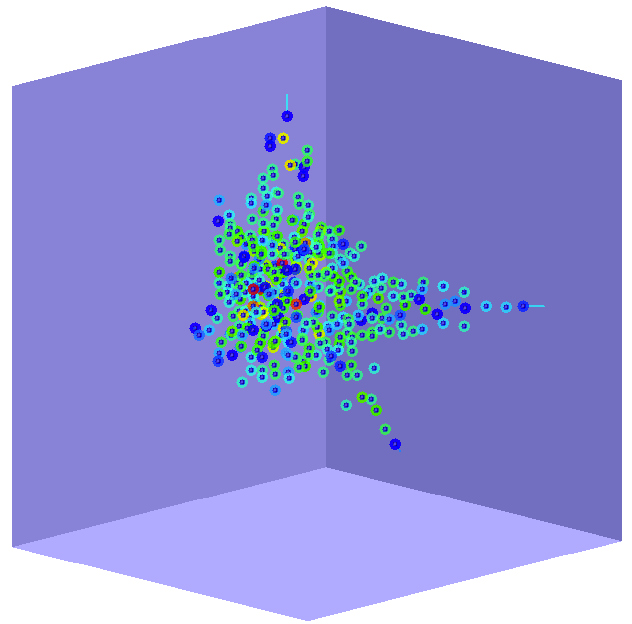
\includegraphics[width=0.95\textwidth]{cascade.png} 

{\tiny \red{unfortunately the last pretty picture for today}}
\end{center}
\end{minipage}
}

%%%%%%%%%%%%%%%%%%%%%%%%%%%%%%%%%%%%%%%%%%%%%%%%%%%%%%%%%%%%%%%%%%%%%%%%%%%%
\section{\,}
%%%%%%%%%%%%%%%%%%%%%%%%%%%%%%%%%%%%%%%%%%%%%%%%%%%%%%%%%%%%%%%%%%%%%%%%%%%%

%\frame{\frametitle{Motivation}

%compositionally and structurally complex materials and processes: deposition (newtonian trajectory until hit) and radiation damage.

%}

%%%%%%%%%%%%%%%%%%%%%%%%%%%%%%%%%%%%%%%%%%%%%%%%%%%%%%%%%%%%%%%%%%%%%%%%%%%%
\section{Basic idea}
%%%%%%%%%%%%%%%%%%%%%%%%%%%%%%%%%%%%%%%%%%%%%%%%%%%%%%%%%%%%%%%%%%%%%%%%%%%%
\frame{\frametitle{Basic idea}

\vskip -0.1in

{\bf Premise:}
we can decompose the system into sub-configurations ({\it clusters}) and if the sub-configurations are sufficiently large the forces on the central atoms are sufficiently accurate, i.e. \blue{\bf locality}

\vskip 0.1in

{\bf Procedure:}
\begin{enumerate}
\item
as dynamics ensues new ({\it query}) configurations are generated and compared to a cluster-force 
database.\item if sufficient stored clusters are close the query cluster the stored forces are interpolated at the query cluster   %   to those in the database the stored forces are used, perhaps using interpolation via radial basis functions
\item otherwise, {\it ab initio} forces are calculated for the new cluster and stored\end{enumerate}

As opposed to the \red{\it globally}-tuned \red{\it empirical} potential, 
%we do not construct a compact surrogate potential energy function, 
we explicitly propogate the system in time using \red{\it locally interpolated} DFT forces. 

\vskip 0.05in

We endow the database with a distance measure that facilitates: (a) fast metric-based \blue{\bf searches} and (b) robust \blue{\bf interpolation} of database information at queries.

}

%%%%%%%%%%%%%%%%%%%%%%%%%%%%%%%%%%%%%%%%%%%%%%%%%%%%%%%%%%%%%%%%%%%%%%%%%%%%
\section{Distance metric}
%%%%%%%%%%%%%%%%%%%%%%%%%%%%%%%%%%%%%%%%%%%%%%%%%%%%%%%%%%%%%%%%%%%%%%%%%%%%

\frame{\frametitle{Cluster distance}
A {\it cluster} $\cluster_A$ is a set 
$
\cluster_A = \{ \dx_{1a}, \dx_{2a}, \dx_{3a}, \ldots, \dx_{N_A a} \}
$
of distance vectors 
$\Delta\xb_{\alpha a} \equiv \xb_\alpha - \xb_a$ 
relative to a central atom $\xb_a$,

\vspace{0.1in}
A distance $d(A,B)$ between clusters $\cluster_A$ \&  $\cluster_B$, needs
(a)
basic \blue{\bf metric} properties:
\begin{enumerate}
\item[M1] {\bf coincidence}:  $d(A,B) = 0 \ \text{iff} \ A=B $
\item[M2] {\bf positivity}:  $d(A,B) > 0 $
\item[M3] {\bf symmetry}: $d(A,B) = d(B,A)$
\item[M4] {\bf triangle inequality}: $d(A,C) \le d(A,B) + d(B,C)$
\item[M5] {\bf reverse triangle inequality}: $d(A,C) \ge | d(A,B) - d(B,C) |$
\end{enumerate}
and (b)  physical \blue{\bf invariances} $d(A,B) = d(A,B')$:
\begin{enumerate}
\item[II] {\bf translation} $\cluster_B \to \cluster_{B'} = \cluster_B + \ab$
\item[I2] {\bf rotation}    $\cluster_B \to \cluster_{B'} = \Rb \cluster_B $
\item[I3] {\bf permutation} $\cluster_B \to \cluster_{B'} = \Pb \cluster_B $
\end{enumerate}

}
%---------------------------------------------------------------------------
\frame{\frametitle{Root Mean Square Distance}

Assuming $N_A = N_B$, the root mean square deviation (RMSD) comparison metric is
\begin{equation}
\begin{split}
d_\text{RSMD}(A,B) 
& %= \min_{\Rb,\Pb} d(\Xs_a, \Rb \Pb \Xs_b)
 = \min_{\Rb,\Pb} \| \Xs_A - \Rb \Pb \Xs_B \|_w  \\
&= \min_{\Rb,\Pb} \sqrt{ \left( \Xs_A - \Rb \Pb \Xs_B\right) \cdot \Ws_{AB} \left( \Xs_A - \Rb \Pb \Xs_B\right) }
 \\
&\equiv
\min_{\Rb,\Pb} \sqrt{ \sum_{\alpha,\beta=1}^{N_b} { \|\dx_{\alpha a} - \Rb P_{\alpha\beta} \dx_{\beta b} \|^2  \
     w_{\alpha \beta} } } %\negthinspace\left(( \| \dx_i)_a\|, \| (\dx_j)_b \| \right) }
\end{split}
\end{equation}

\vskip -0.1in

where:\\
$\red{\bullet}$ $\Xs_A$ and $\Xs_B$ are matrices of the cluster vectors $\Delta \xb_\alpha$, 
\\
$\red{\bullet}$ $\Rb \in \mathsf{Orth^+}$ is a \underline{rotation} of the cluster and
\\
$\red{\bullet}$ $\Pb$ is a \underline{permutation} of the cluster ordering, \\
\ \ \ i.e. a binary orthogonal matrix which is simply the rearrangment of the rows or columns of the identity matrix.

}

%---------------------------------------------------------------------------
\frame{\frametitle{Optimal rotation}

\vskip -0.2in 

\begin{equation*} 
\begin{split}
d(A,B) 
&= \min_{\Rb,\Pb} \sqrt{ \left( \Xs_A - \Rb \Pb \Xs_B\right) \cdot \Ws_{AB} \left( \Xs_A - \Rb \Pb \Xs_B\right) } \\
&= \min_{\Rb,\Pb} \sqrt{ \|\Xs_A\|^2_w + \|\Xs_B\|^2_w - 2 \Xs_A \cdot \Ws_{AB} \Rb \Pb \Xs_B }
 \\
\end{split}
\end{equation*}
To determine the rotation $\Rb$, Kabsch (1976) noticed the last term
\begin{equation*} 
2 \Xs_A \cdot \Ws \Rb \Pb \Xs_B 
%= 2 \tr\left( \Ws(\Xs)\Rb \Pb \Xs_b \Xs_a^T\right)
= 2 \tr\left( \Rb \Pb \Xs_B \Xs_A^T \Ws_{AB} \right)
\end{equation*}
 is the only one dependent on $\Rb$.

\vskip 0.1in

A (3x3) singular value decomposition
$\SVD[ \Pb \Xs_B \Xs_A^T \Ws_{AB}] = \Us \Ds \Vs^T $
gives the solution $\Rb = \Vb \Ub^T$ and
\begin{equation*} 
d(A,B) = \min_{\Pb} \sqrt{ \|\Xs_A\|^2_w + \|\Xs_B\|^2_w - 2 \tr \Db(\Pb)}
\end{equation*}
}

%---------------------------------------------------------------------------
\frame{\frametitle{Distance from Gaussian densities}
Finding the optimal \red{\it permutation} $\Pb$ is considerably harder, requiring e.g. the Hungarian Algorithm.

\vskip 0.1in

As in Bartok (2013), a permutation invariant metric can be formed from atomic densities 

\vskip -0.2in

\begin{equation*}
\rho(\xb) = \Delta(\mathbf{0}) + \sum_\alpha \Delta(\xb - \xb_\alpha) 
= \sum_{\alpha} \sum_{l=0}^\infty \sum_{m=-l}^l c_\alpha^{lm}(r) Y_{lm} (\rb)
\end{equation*}

\vskip -0.1in

represented by a spherical harmonic expansion in $r=\|\xb\|$ and $\rb = \xb/r$, 
where

\vskip -0.2in

\begin{equation*}
\Delta(\xb) = \exp\left(- \frac{ \| \xb - \xb_\alpha \|^2}{2\sigma^2}\right) 
\end{equation*}

\vskip -0.1in

And so 

\vskip -0.2in

$$
d_\text{SOAP}(\rho_A,\rho_B) 
= \sqrt{\frac{S(\rho_A,\rho_A) S(\rho_B,\rho_B) - S(\rho_A,\rho_B)^2}{S(\rho_A,\rho_B)^2}}
$$
where
$ 
S(\rho_A,\rho_B) = \min_\Rb  \int d\xb \, \rho_A(\xb) \rho_B(\Rb \xb) 
$

}

%%%%%%%%%%%%%%%%%%%%%%%%%%%%%%%%%%%%%%%%%%%%%%%%%%%%%%%%%%%%%%%%%%%%%%%%%%%%
\section{Metric search}
%%%%%%%%%%%%%%%%%%%%%%%%%%%%%%%%%%%%%%%%%%%%%%%%%%%%%%%%%%%%%%%%%%%%%%%%%%%%
%---------------------------------------------------------------------------
\frame{\frametitle{Metric database search}

\vskip -0.1in

A key ingredient is searching a large, dense database efficiently

\vskip  0.1in

\begin{minipage}[h!]{0.5\textwidth}
\fbox{
\begin{minipage}[h!]{0.99\textwidth}
\small
\begin{itemize}%[leftmargin=0pt]
%\setlength{\itemindent}{0em}
%\setlength{\listparindent}{0pt}
%\setlength{\leftmargin}{0pt}
\item {\bf Initialize:} \underline{\it select} a set of points $\{R_i\}$ in the database randomly or from previous time step.
%First set is random or uniformly sprinkled all subsequent sets are from history and cached in memory (and deleted if not used)
\item {\bf Loop:}
\begin{enumerate}
\item \underline{\it Find} closest in set:
$\argmin_{R}  d(Q,R_i)$, where Q is the query configuration 
%and $A_n$ is the nth point of the selected points.
%The point $A_m$ is the one with the smallest d(X, $A_m$).
\item \underline{\it Retrieve} neighboring set
$\{N\}$ of points about the point $R$  for which $2 d(N_i,R) < d(Q,R)$
\item \underline{\it Stop} if the neighborhood around $Q$ is the desired radius or size.
\end{enumerate}
\end{itemize}
\end{minipage}
}
\end{minipage}\hfill\hspace{0.1in}%
\begin{minipage}[h!]{0.45\textwidth}
{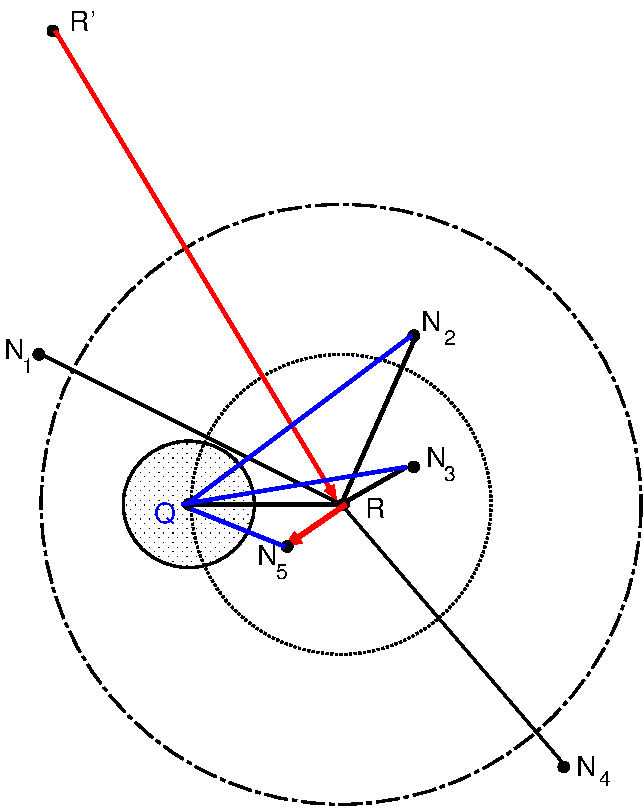
\includegraphics[width=0.9\textwidth]{\figpath/metric_search.pdf}}
{\tiny {\bf Query point} Q, {\bf reference point} R and its neighbors N$_i$ in the database. 
The subset \{  N$_2$, N$_3$, N$_5$ \} are candidates for configurations in the interpolation ball around Q. After computation of distances of the subset to Q, N$_5$ will be selected as the best candidate for the new R.}
\end{minipage}

}
%%%%%%%%%%%%%%%%%%%%%%%%%%%%%%%%%%%%%%%%%%%%%%%%%%%%%%%%%%%%%%%%%%%%%%%%%%%%
\section{Force interpolation}
%%%%%%%%%%%%%%%%%%%%%%%%%%%%%%%%%%%%%%%%%%%%%%%%%%%%%%%%%%%%%%%%%%%%%%%%%%%%
%---------------------------------------------------------------------------
\frame{\frametitle{Interpolation of forces}

\begin{minipage}[h!]{0.5\textwidth}
Given $\{d_{\alpha\beta}\} \ | \ \beta \in \Ball_\alpha$ for $\alpha$ an accurate force $\fb_\alpha$ can be obtained from  simple interpolation
$$
\fb_\alpha = \sum_{\beta\in \Ball_\alpha} \Rb_\beta \fb_\beta \phi(d_{\alpha\beta})
$$
such that $\sum_\beta \phi(d_{\alpha\beta}) = 1$ and $\phi(r) \sim \frac{1}{r}$.

\vskip 0.1in

Here $\Rb_\beta$ is an optimal rotation from the reference cluster $\beta_i$ to the query cluster $\alpha$, obtained by
$$
\argmin_{\Rb} d(C_\alpha,\Rb C_\beta)
$$

\end{minipage}\hfill%
\begin{minipage}[h!]{0.45\textwidth}
\begin{center}
{\bf Cluster space}

\vskip 0.1in

{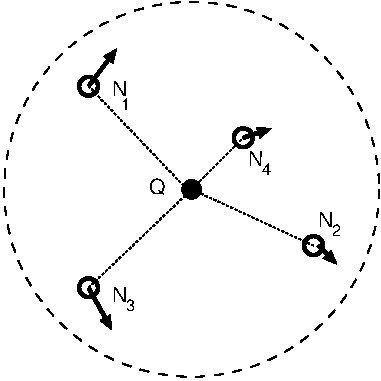
\includegraphics[width=0.99\textwidth]{\figpath/interpolation_schematic.pdf}}

\vskip 0.1in

{\tiny this is the trust ball around the query point Q in the previous slide}
\end{center}
\end{minipage}
}

%%%%%%%%%%%%%%%%%%%%%%%%%%%%%%%%%%%%%%%%%%%%%%%%%%%%%%%%%%%%%%%%%%%%%%%%%%%%
\section{Results}
%%%%%%%%%%%%%%%%%%%%%%%%%%%%%%%%%%%%%%%%%%%%%%%%%%%%%%%%%%%%%%%%%%%%%%%%%%%%
\frame{\frametitle{Convergence of force with cluster size}


\vskip -0.1in

Small atomic displacements produce changes in force on nearby atoms that quickly decay with distance.

\vskip 0.1in

Magnitude of the Hellmann-Feynman force for a 512 atom Si supercell

\begin{center}

Increasing displacement $\Longrightarrow$ 0.037, 0.37 and 3.7 \AA

\fbox
{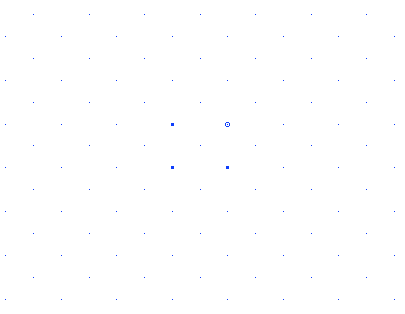
\includegraphics[width=0.3\textwidth]{\figpath/force1.png}}
\fbox
{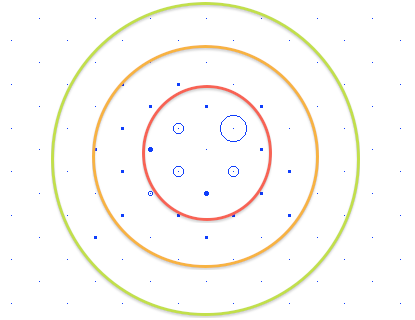
\includegraphics[width=0.3\textwidth]{\figpath/force2.png}}
\fbox
{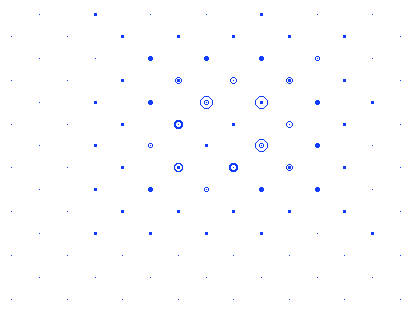
\includegraphics[width=0.31\textwidth]{\figpath/force3.png}}

Increasing forces $\Longrightarrow$  0.02, 0.2 and 0.4 eV/\AA
\end{center}


Error is  $\| \fb_{\text{Ball}(R)} - \fb^* \|$ where $\fb^*$ is the force in the full system.

}
%---------------------------------------------------------------------------
%\frame{\frametitle{Search performance}
%}
%---------------------------------------------------------------------------
\frame{\frametitle{Correlation of cluster distance and forces}
\begin{minipage}[h!]{0.45\textwidth}
The difference in forces on the central atom for two clusters

\vskip -0.2in

$$\| \fb_\alpha - \fb_\beta \|$$

\vskip -0.1in

is highly correlated with with the inter-cluster distance $d_{\alpha\beta}$.

\ \ The \blue{blue} line depicts the probability density - showing that the mostly likely difference is quite peaked.

\ \ Also the candidates for interpolation in the {\bf black} box are separated from the bulk of the clusters.

\ \ The close-up shows that the correlation is quite linear

\end{minipage}\hfill%
\begin{minipage}[h!]{0.5\textwidth}
\begin{center} 
{\tiny vertical: {\bf force similarity}, horizontal: {\bf cluster distance}}

{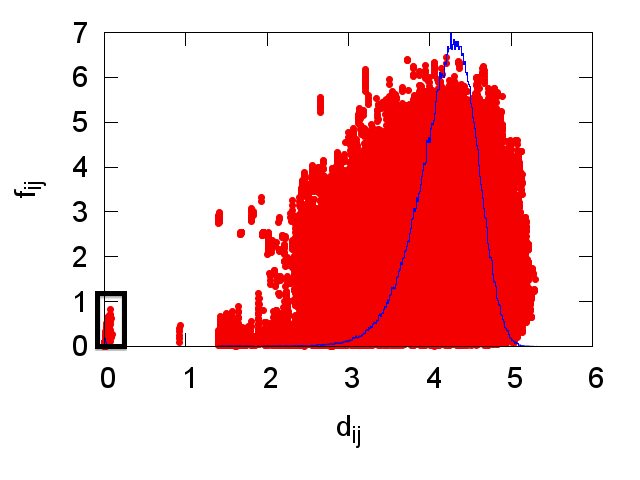
\includegraphics[width=0.95\textwidth]{f-d_block_12.png}}

{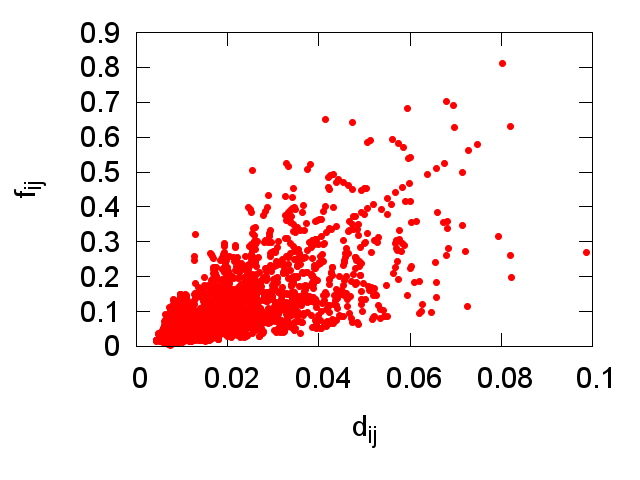
\includegraphics[width=0.95\textwidth]{\figpath/f-d_closeup_block_12.png}}
\vskip -0.35in
{\bf $\Longleftarrow$ better match}
\end{center}
\end{minipage}

}
%---------------------------------------------------------------------------
\frame{\frametitle{Sensitivity to the cluster size}
\begin{center}
Force-distance correlation for increasing cluster size $\Longrightarrow$

\vskip 0.2in

\fbox
{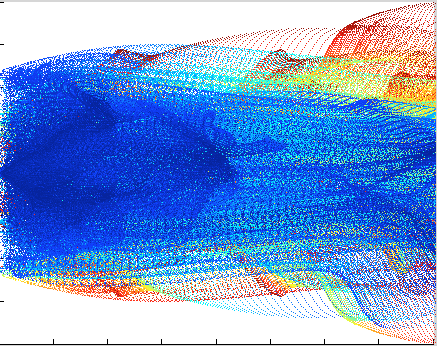
\includegraphics[width=0.3\textwidth]{FvsD_2neighbs.png}}
\fbox
{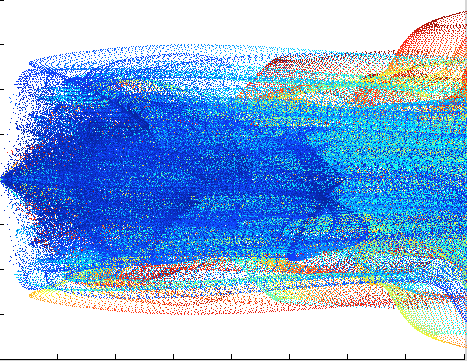
\includegraphics[width=0.3\textwidth]{FvsD_4neighbs.png}}
\fbox
{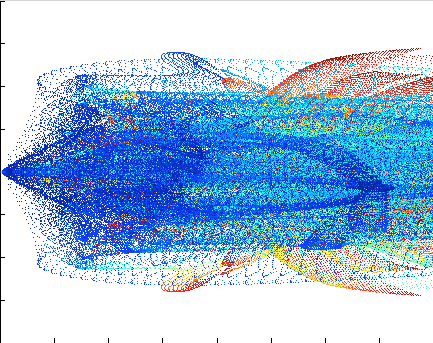
\includegraphics[width=0.3\textwidth]{FvsD_6neighbs.png}}

vertical: force similarity, horizontal: cluster distance
\end{center}

\vskip 0.2in

Notice the peak that forms at $(d_{\alpha\beta},\| \fb_\alpha - \fb_\beta \|) = (0,0)$ as the cluster size increases, i.e. the metric becomes more discriminating as the number of neighboring atoms included in the metric increases.
}
%---------------------------------------------------------------------------
\frame{\frametitle{Metric search efficiency}

\vskip -0.05in

Measuring search efficiency as: (s-d)/s where $s$=database size \& $d$=number of distance computations 

\vskip -0.1in

\begin{center}
{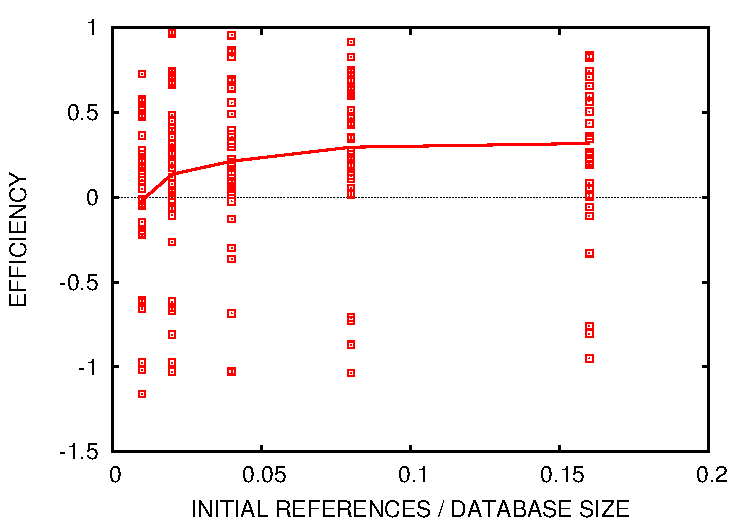
\includegraphics[width=0.65\textwidth]{metric_search_efficiency.pdf}}
\end{center}

\vskip -0.1in

As the number of initial {\it reference} clusters, clusters chosen for \underline{new} calculations of distance to the query cluster, increases the metric search becomes more efficient. 
This trend has a obvious limit as the entire database is sampled by the initial set of reference clusters
}

%%%%%%%%%%%%%%%%%%%%%%%%%%%%%%%%%%%%%%%%%%%%%%%%%%%%%%%%%%%%%%%%%%%%%%%%%%%%
\section{Conclusion}
%%%%%%%%%%%%%%%%%%%%%%%%%%%%%%%%%%%%%%%%%%%%%%%%%%%%%%%%%%%%%%%%%%%%%%%%%%%%
\frame{\frametitle{Current work}

%\vskip -0.2in

%\hspace{0.6\textwidth} {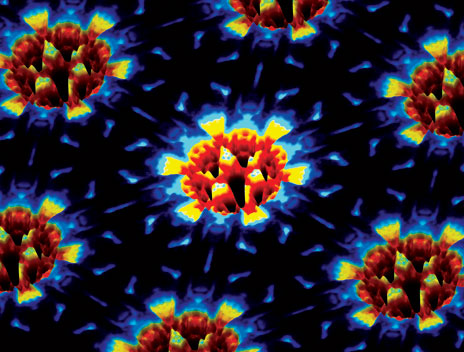
\includegraphics[width=0.3\textwidth]{topo_insulator.jpg}}

\begin{itemize}
%\begin{minipage}[t]{0.5\textwidth}
\item We have results for the dynamics of  1- and 3-D test systems but they are aren't that interesting since we have only been testing consistency of the method and full {\it ab initio} and classical molecular dynamics.
\end{itemize}

\begin{minipage}[c]{0.6\textwidth}
\begin{itemize}
\item 
Application to atomic deposition, radiation damage, and structurally interesting materials like topological insulators is upcoming
\end{itemize}
\end{minipage}\hfill% \hspace{0.1in}  %\hfill%
\begin{minipage}[c]{0.28\textwidth}
%{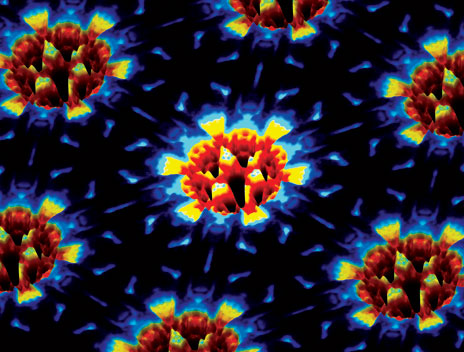
\includegraphics[width=0.95\textwidth]{topo_insulator.jpg}}
{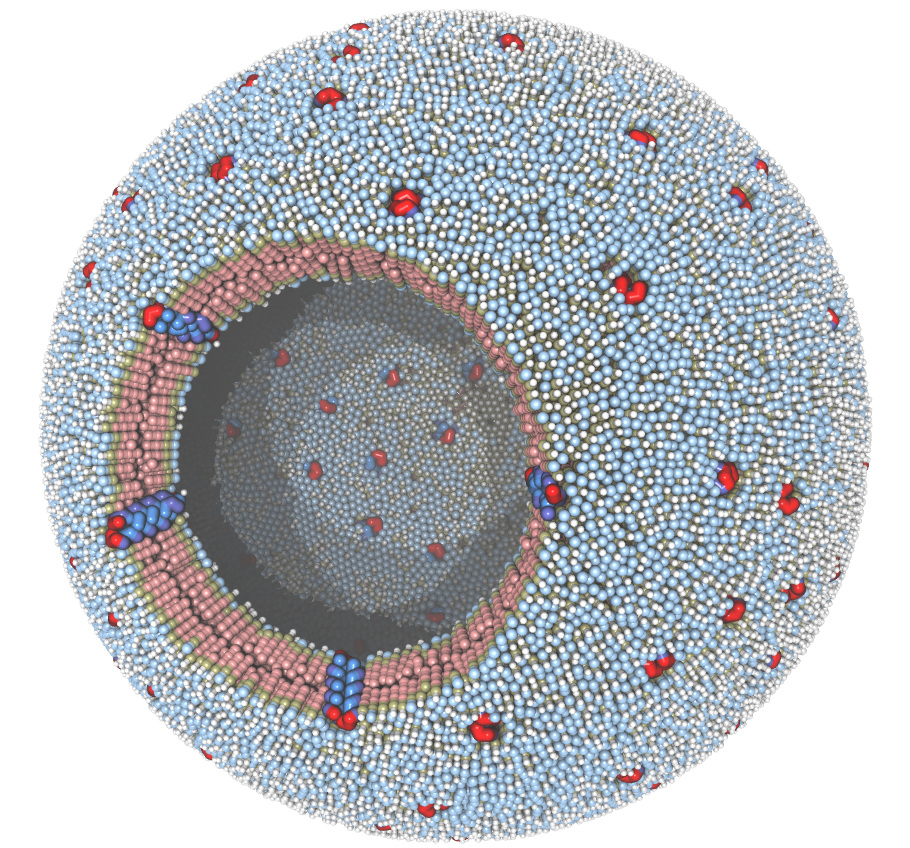
\includegraphics[width=0.95\textwidth]{vesicle_membrane+protein.jpg}}
\end{minipage}

\begin{itemize}

\item Since the method reduces to {\it ab initio} molecular dynamics in the limit to full system clusters and no interpolation, we are trying to make stronger connections to it

\item We are also exploring using machine learning techniques to enhance the search and interpolation methodology.
\end{itemize}

\begin{center}
Reese Jones \blue{\bf rjones@sandia.gov}
\end{center}
}

\end{document}


Randomly generated database – just configurations, no forces. 
N = 400 configs, Nneighb= 4, Nsample =  10, Nref = 4
RMSD operations = {382, 311, 257, 128, stuck, 336,  423, 281, 402, 249 (missed by 0.004), 320 (missed by 0.1), 371, 256 (missed by 0.012), 400}
SOAP operations = {664,404, stuck, stuck, stuck, 455, 125, stuck, 148,    
N = 800 configs, Nneighb= 4, Nsample =  10, Nref = 8
RMSD operations = {750, 611, 848, 821, 1050, 438 (missed by 0.04), 482 (missed by 0.02), 218, 759, 290}
N = 800 configs, Nneighb= 4, Nsample =  10, Nref = 40
RMSD operations = {486, 458, 310, 682, 337, 86, 399, 397, 456, 85}
N = 2000 configs, Nneighb= 5, Nsample =  10, Nref = 100
RMSD operations = {869, 299, 299 (missed by 0.05), 494, 177, 1284, 1732, 1486, 1017, 472, 803}
N = 800 clusters, Nneighb= 6, Nsample =  10. Nref = 8
RMSD operations = {516, 427, 602, 108, 825, 997, 648, 951, 408, 584}
N = 800 clusters, Nneighb= 6, Nsample =  10. Nref = 16
RMSD operations ={277, 549, 763, 84, 905, 320, 872, 907, 612, 53}
Results sensitive to tolerance and number of reference clusters. If tolerance is too low, the search gets ‘stuck’, if its too high it misses. 

